\begin{figure}[h!]
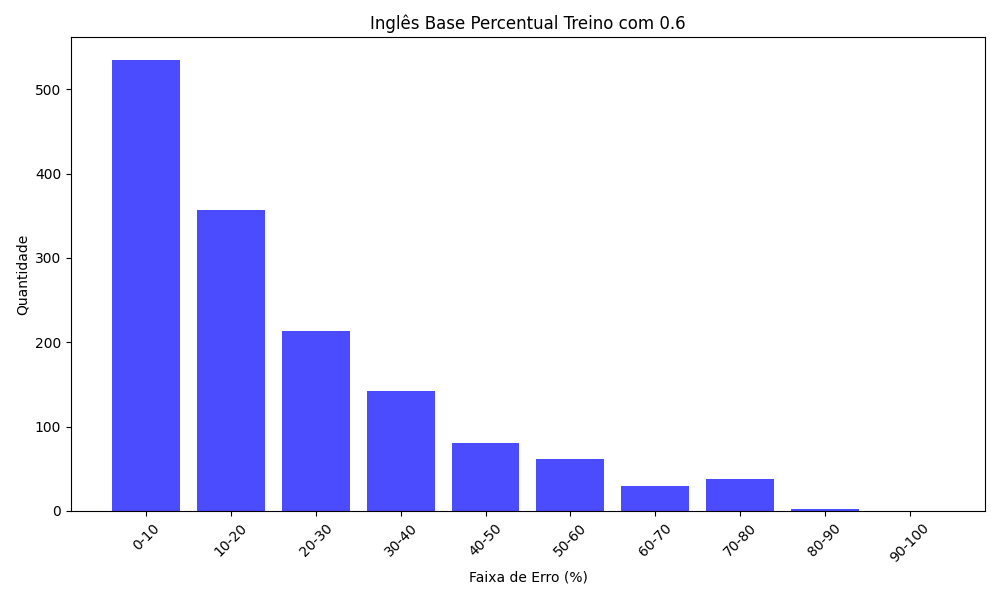
\includegraphics[width=\textwidth]{img/grafsEng/Inglês Base Percentual Treino com 0.6_quantidade.png}
\caption{Quantidade de respostas por faixas de erro percentual dos testes com 40\% do \textit{dataset Mohler} (Inglês) usando o Modelo \textit{BERT Base}}\label{figure:16}
\end{figure}

\begin{figure}[h!]
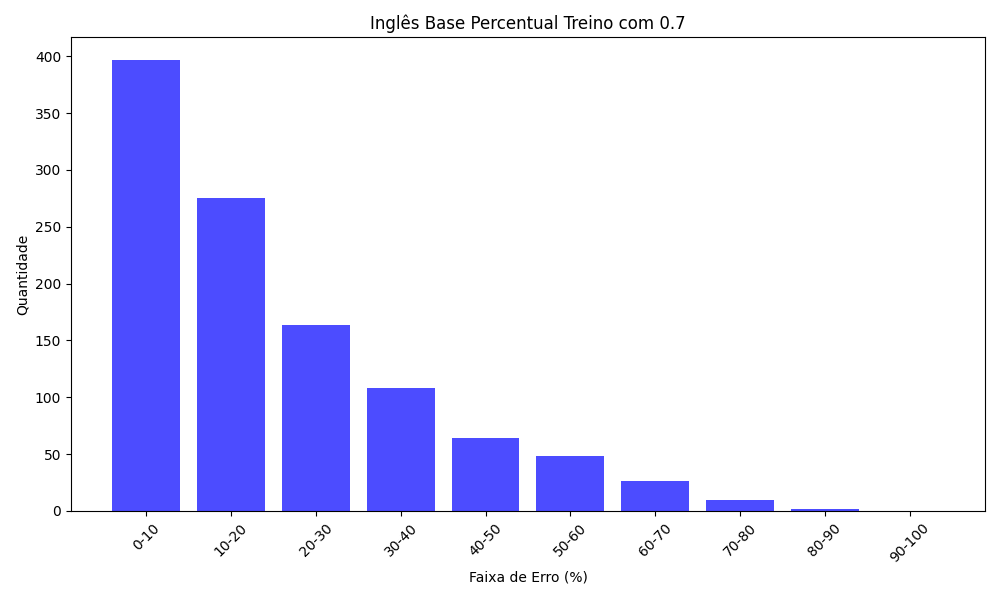
\includegraphics[width=\textwidth]{img/grafsEng/Inglês Base Percentual Treino com 0.7_quantidade.png}
\caption{Quantidade de respostas por faixas de erro percentual dos testes com 30\% do \textit{dataset Mohler} (Inglês) usando o Modelo \textit{BERT Base}}\label{figure:17}
\end{figure}

\begin{figure}[h!]
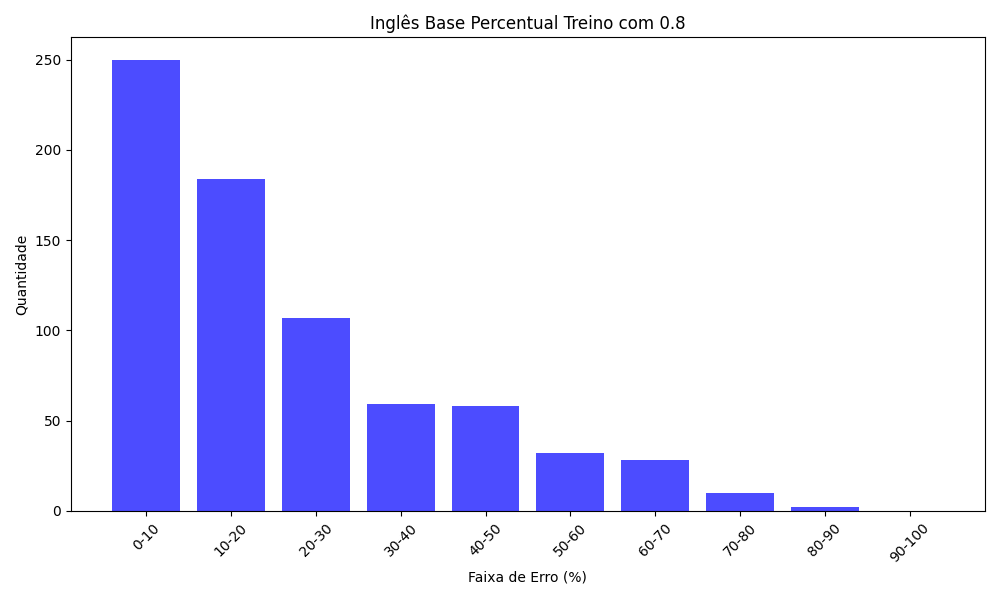
\includegraphics[width=\textwidth]{img/grafsEng/Inglês Base Percentual Treino com 0.8_quantidade.png}
\caption{Quantidade de respostas por faixas de erro percentual dos testes com 20\% do \textit{dataset Mohler} (Inglês) usando o Modelo \textit{BERT Base}}\label{figure:18}
\end{figure}

\begin{figure}[h!]
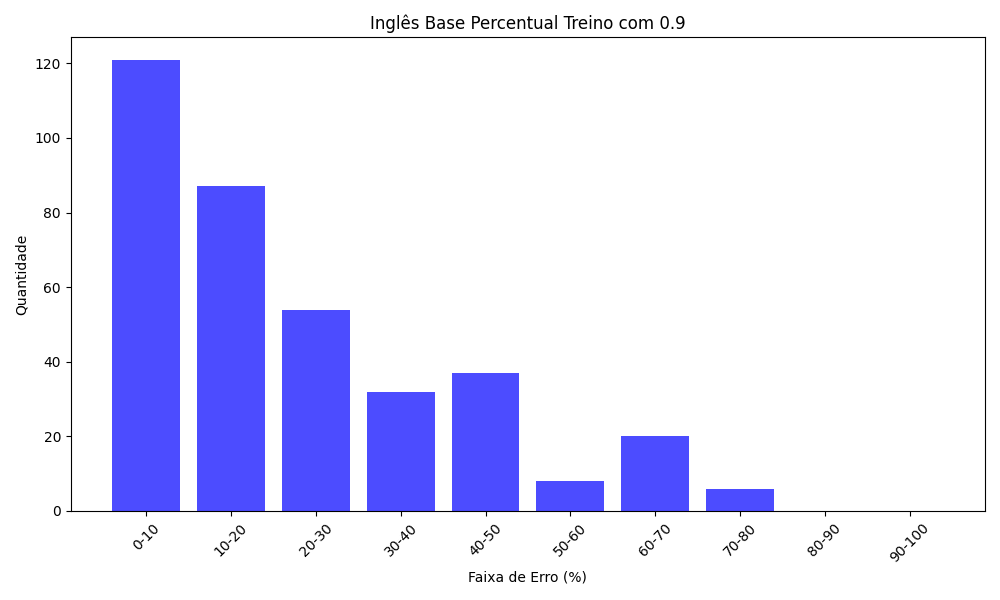
\includegraphics[width=\textwidth]{img/grafsEng/Inglês Base Percentual Treino com 0.9_quantidade.png}
\caption{Quantidade de respostas por faixas de erro percentual dos testes com 10\% do \textit{dataset Mohler} (Inglês) usando o Modelo \textit{BERT Base}}\label{figure:19}
\end{figure}